% !TEX encoding = UTF-8 Unicode
\documentclass[a4paper, 11pt, nofonts, nocap, fancyhdr, hyperref, UTF8]{ctexart}

\usepackage[margin=90pt]{geometry}
\usepackage{amsfonts}
\usepackage{amsthm}
\usepackage{indentfirst}             % 首行缩进
\usepackage[perpage,symbol]{footmisc}% 脚注控制
\usepackage[sf]{titlesec}            % 控制标题
\usepackage{titletoc}                % 控制目录
\usepackage{fancyhdr}                % 页眉页脚
\usepackage{type1cm}                 % 控制字体大小
\usepackage{indentfirst}             % 首行缩进
\usepackage{makeidx}                 % 建立索引
\usepackage{textcomp}                % 千分号等特殊符号
\usepackage{layouts}                 % 打印当前页面格式
\usepackage{bbding}                  % 一些特殊符号
\usepackage{cite}                    % 支持引用
\usepackage{color,xcolor}            % 支持彩色文本、底色、文本框等
\usepackage{listings}                % 粘贴源代码
\usepackage{algorithm,algpseudocode, algorithmicx}
%\usepackage{algorithmic}
\usepackage{graphics}
\usepackage{graphicx}
\usepackage{epsfig}
%\usepackage[dvips]{graphicx}       % 将eps格式的图片放在figures目录下
%\usepackage[pdftex]{graphicx}      % \graphicspath{{figures/}}
\usepackage{multirow}
\usepackage{amsmath}
\usepackage{amstext}
%\usepackage[colorlinks,linkcolor=red]{hyperref}
\usepackage{subfigure}
\usepackage{float} %算法浮动体
\usepackage{xeCJK} % 使用xeCJK宏包

\lstloadlanguages{}                  % 所要粘贴代码的编程语言

\setCJKmainfont[Mapping = fullwidth-stop, BoldFont={黑体-简}, ItalicFont={楷体-简}]{宋体-简}
\setCJKsansfont[Mapping = fullwidth-stop, BoldFont={黑体-简}, ItalicFont={楷体-简}]{宋体-简}
\setCJKmonofont[Mapping = fullwidth-stop, BoldFont={黑体-简}, ItalicFont={楷体-简}]{宋体-简}
%\setCJKmainfont{宋体}
%\setCJKsansfont{宋体}
%\setCJKmonofont{宋体}

\titleformat*{\section}{\Large \bf}
\titleformat*{\subsection}{\large \bf}

\CTEXoptions[today=small]

\pagestyle{plain}

\newtheorem{example}{例}[section]             % 整体编号
\newtheorem{theorem}{定理}[section]  % 按 section 编号
%\newtheorem{proof}{证明}[section]
\newtheorem{definition}{定义}[section]
\newtheorem{axiom}{公理}
\newtheorem{property}{性质}
\newtheorem{proposition}{命题}
\newtheorem{lemma}{引理}
\newtheorem{corollary}{推论}
\newtheorem{remark}{注解}
\newtheorem{condition}{条件}
\newtheorem{conclusion}{结论}
\newtheorem{assumption}{假设}
\floatname{algorithm}{算法}

\renewcommand{\contentsname}{目录}     % 将Contents改为目录
\renewcommand{\abstractname}{摘\ \ 要} % 将Abstract改为摘要
\renewcommand{\refname}{参考文献}      % 将References改为参考文献
\renewcommand{\indexname}{索引}
\renewcommand{\figurename}{图}
\renewcommand{\tablename}{表}
\renewcommand{\appendixname}{附录}
\renewcommand{\baselinestretch}{1.3}

\DeclareMathOperator{\argmin}{argmin}
%\DeclareMathOperator{\Im}{Im}
%\DeclareMathOperator{\Ker}{Ker}

\begin{document}

\title{抓取剪切GrabCut——交互式迭代前景分离算法}

\author{\small{数字信号处理期末作业}\\
傅长青\ 卢川\\
}
\date{\today}
\maketitle

\begin{abstract}% 不缩进
本论文实现了Rother et al. 2004年的前景分割算法\cite{rother2004grabcut},大体是总结了以往的若干算法,特别是贝叶斯聚类算法Bayes Matting (Chuang et al. 2001, Ruzon and Tomasi 2000),和图像切割算法Graph Cut (Boykov and Jolly 2001; Greig et al. 1989),并做出了一些创新,包括“迭代优化”和“不完全标记”。此算法主要应用统计模型中的EM算法,以及一些统计物理的思想。
\end{abstract}

\section{引言}
\subsection{以往研究}
Magic wand; Intelligent scissors; Bayes matting(提出了Trimap模型); Knockout 2; Graph Cut(和Bayes matting类似,包括Trimap和概率颜色模型。将在section 2详细说明。这种方法可以处理前景背景渐进色); Level sets等。

\subsection{抓取剪切Grabcut:}
\subsubsection{符号定义}
$T = \{T_B, T_F, T_U\}$ Trimap; $T_B$: Background, $T_F$: Foreground, $T_U$: Undecided 

$z = (z_1,\ldots,z_N)$图像灰度值

$\underline{\alpha} = (\alpha_1,\ldots,\alpha_N)$: 前景的可能性。$\alpha \in \{0,1\}$为硬分割,$\alpha \in [0,1]$为一般情况

$\underline{\theta} = \{h(z; \alpha); \alpha = 0,1, \int_z h(z; \alpha) = 1\}$图像前景背景的灰度值分布。由灰度值的频率(histogram)组成。

$U(\underline{\alpha},\underline{\theta},z) := \sum_n -\log h(z_n, \alpha_n)$已知灰度分布频率$\underline{\theta}$时,$\underline{\alpha}$对数据$z$的拟合程度。

$V(\underline{\alpha},z) := \gamma \sum_{(m,n \in C)} \|m-n\|^{-1}[\alpha_m \neq \alpha_n]  \exp (-\beta(z_m - z_n)^2)$  描述图像的光滑程度。其中$C$是相邻像素对(回忆扫雷游戏),$[\alpha_m \neq \alpha_n] := \text{\Large 1}_{\alpha_m \neq \alpha_n}(m,n)$,$\gamma$是常数

\subsubsection{思路}
理想情况下,使$\alpha$值在$T_U$上连续,不加以$\alpha$只能取0或1这样的限制。这样一来烟雾、头发之类的物体可以自动处理。然而这样的一般方法(Ruzon 2000,Chuang 2001)会造成保护色或靠近颜色下的误判情况。故我们使用下列步骤一步一步抓取前景。

首先考虑硬分割($\alpha \in {0,1}$),使用迭代Graph Cut方法(Section 2,3),其次用边界聚类计算一个窄带(Section 4)。Grabcut并不处理边缘之外的完全透明区域,如果要处理可以用Matting Brush(Chuang 2001)方法,但据经验这种方法还是只能处理边界分明的情况。

Grabcut的创新在于用了两个方法:迭代估计和不完全标记。以及使用了一个计算$\alpha$值的新方法用于边界聚类。

\section{基于Graph Cut的图像分割}
分割的目标是从$z$和$\underline{\theta}$推断未知的$\underline{\alpha}$。定义Gibbs能量:
$$
\textbf{E}(\underline{\alpha},\underline{\theta},\textbf{z}) = U(\underline{\alpha},\underline{\theta},\textbf{z})+V(\underline{\alpha},\textbf{z})
$$
其中,
$U(\underline{\alpha},\underline{\theta},z) := \sum_n -\log h(z_n, \alpha_n)$
是已知灰度分布频率$\underline{\theta}$时,$\underline{\alpha}$对数据$z$的拟合程度。
$\beta = 0$(处处视为光滑)时为所谓的的Ising先验。这里我们取$\beta = (2\mathbb{E}(z_m-z_n)^2)^{-1}$(Boykov and Jolly 2001)。
然后取全局最小为划分的估计:
$$
\hat{\underline{\alpha}} = \arg \min \limits_{\underline{\alpha}} \textbf{E}(\underline{\alpha},\underline{\theta})
$$
首先,用混合高斯分布模型(GMM)代替灰度出现频率;第二,将单次最小切割算法用迭代算法代替。第三,需要用户交互解决的地方用不完全标记法即可放宽要求,即用套索或一个长方形将物体框住即可。

\section{GrabCut 分割算法}
分为迭代估计(译注:一般称为EM算法)和不完全标记两个部分。下面开始像素空间为RGB彩色,采取软分割的方法(Ruzon2000; Chuang 2001)

定义$\textbf{k} = \{k_1,\ldots,k_N\}$现在Gibbs能量变成:
$$
\textbf{E}(\underline{\alpha},\textbf{k},\underline{\theta},z) = U(\underline{\alpha},\textbf{k},\underline{\theta},\textbf{z})+V(\underline{\alpha},\textbf{z})
$$
$U$是$K$元混合高斯模型(GMM),K一般取5即可。
$$
U(\underline{\alpha},\underline{\theta},z) := \sum \limits_n \limits^K D(\alpha_n,k_n,\underline{\theta},z_n) \\
$$
其中
\begin{eqnarray}
&&D(\alpha_n,k_n,\underline{\theta},z_n)\nonumber\\
&=&-\log p(z_n|\alpha_n,k_n,\underline{\theta})-\log\pi(\alpha_n,k_n) \nonumber\\
&=& -\log \pi(\alpha_n,k_n)+\frac{1}{2}\log\det \Sigma(\alpha_n,k_n)+\frac{1}{2}[z_n-\mu(\alpha_n,k_n)]^T\Sigma(\alpha_n,k_n)^{-1}[z_n-\mu(\alpha_n,k_n)]\nonumber
\end{eqnarray}
$p$是高斯分布密度函数,$\pi$是混合分布权值系数。现在系数$\underline{\theta}$为:
$$
\underline{\theta} = \{\pi(\alpha,k), \mu(\alpha,k), \Sigma(\alpha,k), \alpha = 0,1, k = 1,\ldots,K\}
$$
光滑项:
$$
V(\underline{\alpha},z) := \gamma \sum_{(m,n \in C)} [\alpha_m \neq \alpha_n]  \exp (-\beta \|z_m - z_n\|^2)
$$

\begin{algorithm}
\caption{GrabCut}\label{GC}
\textbf{初始化:}\\用户给定$T_B$,设定$T_F = \emptyset$,$T_U = \overline{T_B}$,$n \in T_B$处$\alpha_n = 0$,$n \in T_U$处$\alpha_n = 1$\\
\textbf{迭代步骤:}\\
1.$k_n := \arg \min \limits{k_n} D_n(\alpha_n,\k_n,\theta, z_n)$\\
2.$\underline{\theta}=\arg \min \limits_{\underline{\theta}} U(\underline{\alpha},\textbf{k},\underline{\theta},z)$\\
3.$\{\alpha_n:n \in T_U\} = \arg \min \limits_{\textbf{k}} \textbf{E}(\underline{\alpha},\textbf{k},\underline{\theta},z)$\\
4.重复 Step 1.\\
\textbf{用户交互}\\
编辑:固定一些像素的$\alpha$值为0(称作背景刷)或1(前景刷),运行一次Step 3。\\
提炼:(可选步骤)进行整个迭代步骤。
\end{algorithm}

注:论文后面还讨论了透明像素点的处理,不属于GrabCut算法范畴,故略去不讨论。

\section{实验结果}
采用OpenCV\cite{bradski2008learning} x Python,实验结果如下,示例采用了著名的Lena(credit: shot by photographer Dwight Hooker, cropped from the centerfold of the November 1972 issue of Playboy magazine.):
\begin{figure}[!h]
    \centering
    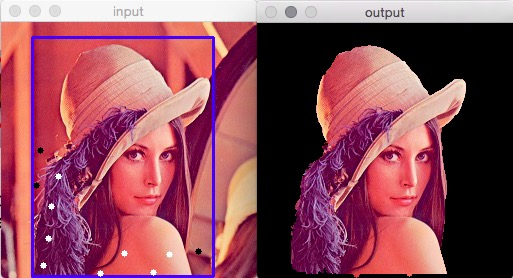
\includegraphics[width=0.7\textwidth]{figures/lena.jpg}
    \caption{实验结果}
\end{figure}

\section{总结与感想}
目前图像处理的研究中(参考http://ipol.im)除了分解算法外,也有不少基于统计学习方法这也是这篇报告采用的方法。今后的学习中我们将会尝试信号处理等方法解决相关问题。

\bibliographystyle{plain}
\bibliography{mybib}


\end{document}
